% Risk Lab: IRRBB of a synthetic bank - draft.
% Figures and tables are generated by report/build_report.py --doc irrbb (synthetic data only).
% Every \usertext{...} is an open prose slot for the author; a build with open slots is a draft.
\documentclass[11pt,a4paper]{article}
\usepackage[a4paper,margin=2.3cm]{geometry}
\usepackage{graphicx}
\usepackage[dvipsnames]{xcolor}
\usepackage{booktabs}
\usepackage{array}
\usepackage{amsmath,amssymb}
\usepackage{caption}
\usepackage{float}
\usepackage[hidelinks]{hyperref}
\captionsetup{font=small,labelfont=bf}
\graphicspath{{./}}

% Reproducible PDF: no creation date, empty trailer ID (pdfTeX primitives).
\ifdefined\pdfinfoomitdate \pdfinfoomitdate=1 \fi
\ifdefined\pdftrailerid \pdftrailerid{} \fi

% ---- open text slots ---------------------------------------------------------------
\newcounter{usertextslots}
\newcommand{\usertext}[1]{%
  \stepcounter{usertextslots}%
  \par\medskip\noindent
  \fcolorbox{BurntOrange}{Goldenrod!18}{\parbox{\dimexpr\linewidth-2\fboxsep-2\fboxrule\relax}{%
    \small\textbf{\textcolor{BurntOrange}{TEXT SLOT \theusertextslots:}} \textit{#1}}}%
  \par\medskip}
\makeatletter
\AtEndDocument{\immediate\write\@auxout{\string\gdef\string\totalusertextslots{\theusertextslots}}}
\makeatother
\providecommand{\totalusertextslots}{?}

\title{Interest rate risk in the banking book of a synthetic bank\\[0.3em]
  \large EVE and NII under the standardised shock scenarios, the outlier tests and the NMD model risk}
\author{}
\date{}

\begin{document}
\maketitle
\vspace{-2em}
\usertext{Author, function and date of the analysis.}
\begin{center}
\fcolorbox{BrickRed}{BrickRed!8}{\parbox{0.9\linewidth}{\centering\small
\textbf{DRAFT} -- this version has \totalusertextslots{} open text slots (orange boxes).
All figures and tables are generated from synthetic data by \texttt{report/build\_report.py --doc irrbb}.}}
\end{center}
\tableofcontents

% =====================================================================================
\section{Executive summary}
Interest rate risk in the banking book (IRRBB) is the risk to a bank's economic value and earnings from
changes in interest rates. Supervisors measure it with six standardised shock scenarios and two outlier tests:
the change in the economic value of equity ($\Delta$EVE) and the change in net interest income ($\Delta$NII),
each against Tier 1 capital. This document applies them to a synthetic retail bank with a known balance sheet
and a known yield curve, and measures how much the answer depends on the modelling of non-maturity deposits
(NMD), the classic model-risk point of IRRBB. The findings are in Table~\ref{tab:R4_findings}; their
severities are proposals.
\usertext{The overall conclusion for the (synthetic) bank in two or three sentences, with the finding IDs.}

% =====================================================================================
\section{Scope and sources}
\begin{itemize}
\item \textbf{Measures:} PV, duration, convexity, DV01 and key-rate DV01s; $\Delta$EVE on run-off cash flows
  (equity excluded); $\Delta$NII over 12 months for a constant balance sheet; the supervisory outlier tests.
\item \textbf{Scenarios:} parallel up / down, steepener, flattener, short up / down, with the shapes and EUR shock
  sizes of the BCBS standard (2016, d368) and its 2024 recalibration (d578, effective 1 January 2026), and the
  post-shock floor of the EBA regulatory technical standards on supervisory outlier tests (EBA/RTS/2022/10, now
  Delegated Regulation (EU) 2024/856); the EU floor is applied to both sets of shock sizes.
\item \textbf{Thresholds:} EVE decline above 15\,\% of Tier 1 over the six scenarios (CRD Art.~98(5)); NII decline
  above 5\,\% of Tier 1 over parallel up / down (Delegated Regulation (EU) 2024/856 Art.~6). Both are parameters.
\item \textbf{Not covered:} credit spread risk (CSRBB), options other than the NMD pass-through (no prepayment or
  early-redemption models), several currencies (and the BCBS weighting of gains across them), behavioural models
  estimated from data, and the full EBA standardised approach.
\end{itemize}
Every parameter and modelling choice with its source is listed in the assumptions register
(Table~\ref{tab:R3_assumptions}); only the NMD caps could not be checked against a primary source and are marked
as an assumption.
\usertext{Which regulatory regime the analysis is meant to mirror (BCBS, EBA, a national supervisor) and which
open assumptions must be verified before any use.}

% =====================================================================================
\section{Method}
\subsection{Yield curve}
Zero rates are continuously compounded and follow the Nelson--Siegel form
$z(t) = \beta_0 + \beta_1 \frac{1-e^{-t/\tau}}{t/\tau} + \beta_2\left(\frac{1-e^{-t/\tau}}{t/\tau} - e^{-t/\tau}\right)$
(Svensson adds a second hump). The base curve of the study has known parameters
($\beta_0 = 3\,\%$, $\beta_1 = -1.5\,\%$, $\beta_2 = 1\,\%$, $\tau = 2$); the library also fits NS / NSS curves to
zero rates or par yields and generates synthetic curves from a dynamic Nelson--Siegel model.

\subsection{Shock scenarios}
With $S_{\text{short}}(t) = R_{\text{short}}\, e^{-t/4}$ and $S_{\text{long}}(t) = R_{\text{long}}(1 - e^{-t/4})$,
the scenarios are $\pm R_{\text{parallel}}$, $\pm S_{\text{short}}$, the steepener
$-0.65\,|S_{\text{short}}| + 0.9\,|S_{\text{long}}|$ and the flattener $+0.8\,|S_{\text{short}}| - 0.6\,|S_{\text{long}}|$.
Shocked rates are floored at $\min(0, -150\text{ bp} + 3\text{ bp} \cdot t)$, or at the observed rate if that is
lower (EBA/RTS/2022/10 Art.~4(k)). The study applies this EU floor to both the 2016 and the 2024 shock sizes.

\begin{figure}[H]
\centering
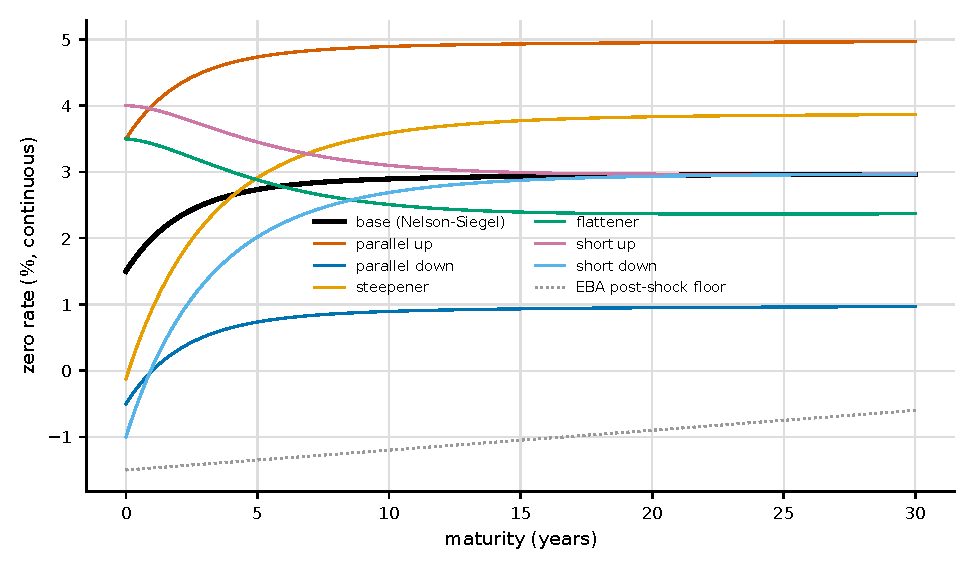
\includegraphics[width=\linewidth]{figures/fig13_irrbb_curves.pdf}
\caption{The synthetic base zero curve (Nelson-Siegel, parameters in the results file) and the six standardised shock scenarios with the EUR shock sizes 200 / 250 / 100 bp (parallel / short / long, BCBS 2016), after the EBA post-shock floor (dotted). Synthetic curve, no market data.}
\label{fig:fig13_irrbb_curves}
\end{figure}


\subsection{Balance sheet and behavioural assumptions}
The reference bank holds EUR 1000\,m of assets (10-year annuity mortgages, 5-year corporate loans, 5- and
10-year government bonds, floating-rate loans, central-bank reserves) funded by current accounts and savings
(non-maturity deposits), term deposits, a covered bond and equity; Tier 1 is 9\,\% of assets. Non-maturity
deposits are modelled by a replicating portfolio: the non-core share runs off overnight, the core share in equal
monthly tranches whose average maturity is a parameter; deposit rates follow market rates with a pass-through
$\beta$ (0.3 for current accounts, 0.5 for savings) and are floored at zero. $\Delta$NII assumes a constant balance
sheet: maturing and repricing balances are replaced by the same product at the shocked rate. These are choices of the
synthetic bank, as are the composition and a Tier 1 of 9\,\% of assets, which is generous for a retail bank.
\usertext{Is the reference composition representative for the bank you have in mind? Which deposit assumptions
would you defend in front of a supervisor?}

% =====================================================================================
\section{Results}
\subsection{EVE and NII per scenario}
\begin{table}[H]
\centering
\scriptsize
\caption{Delta EVE (run-off, equity excluded) and Delta NII (12 months, constant balance sheet) of the synthetic reference bank per standardised scenario, in EUR m and in \% of Tier 1 (90); EUR shock sizes (parallel / short / long, bp): EUR BCBS2016 200 / 250 / 100; EUR BCBS2024 225 / 350 / 200. Deterministic (no Monte-Carlo error).}
\label{tab:R1_scenarios}
\setlength{\tabcolsep}{3pt}
\begin{tabular}{lrrrrrrrr}
\toprule
Scenario & $\Delta$EVE$_{2016}$ & \%T1$_{2016}$ & $\Delta$NII$_{2016}$ & \%T1$_{2016}$ & $\Delta$EVE$_{2024}$ & \%T1$_{2024}$ & $\Delta$NII$_{2024}$ & \%T1$_{2024}$ \\
\midrule
parallel up & -15.8 & -17.6 & +2.75 & +3.1 & -17.6 & -19.6 & +3.10 & +3.4 \\
parallel down & +19.4 & +21.5 & -5.75 & -6.4 & +22.1 & +24.5 & -6.62 & -7.4 \\
steepener & -7.2 & -8.0 & -3.57 & -4.0 & -14.2 & -15.8 & -5.29 & -5.9 \\
flattener & +4.8 & +5.3 & +2.17 & +2.4 & +10.0 & +11.1 & +2.96 & +3.3 \\
short up & -0.5 & -0.5 & +2.88 & +3.2 & -0.7 & -0.7 & +4.04 & +4.5 \\
short down & +0.5 & +0.5 & -6.62 & -7.4 & +0.6 & +0.6 & -9.01 & -10.0 \\
\bottomrule
\end{tabular}
\end{table}

\begin{figure}[H]
\centering
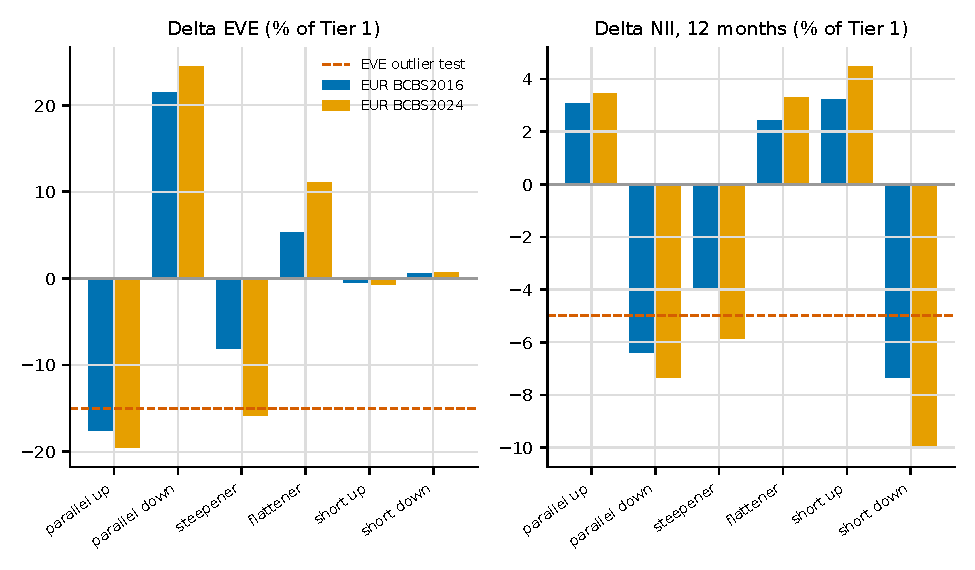
\includegraphics[width=\linewidth]{figures/fig14_irrbb_delta.pdf}
\caption{Delta EVE (run-off, equity excluded) and Delta NII (12 months, constant balance sheet) of the synthetic reference bank per scenario, in \% of Tier 1, for the BCBS 2016 and 2024 EUR shock sizes. Dashed: the supervisory outlier thresholds (15\,\% EVE decline over the six scenarios; 5\,\% NII decline, tested on parallel up / down only).}
\label{fig:fig14_irrbb_delta}
\end{figure}

The bank loses economic value when rates rise (long fixed-rate assets, short funding) and loses income when they
fall (deposit rates cannot fall below zero). The 2024 shock sizes are larger and increase both exposures.

\subsection{Supervisory outlier tests}
\begin{table}[H]
\centering
\scriptsize
\caption{Supervisory outlier tests of the reference bank: the largest EVE decline over the six scenarios against 15\,\% of Tier 1, and the largest NII decline over parallel up / down against 5\,\% of Tier 1 (both thresholds are parameters). Last two columns: share of outliers among 2000 variants of the reference bank (notionals $\times$ U(0.7, 1.3), fixed rates $\pm$ 50 bp; same NMD rates, betas and deposit floor, Tier 1 = 9\,\% of assets), \% $\pm$ Monte-Carlo se; a rate of 0 or 100 shows the 95\,\% bound of the rule of three in brackets.}
\label{tab:R2_outlier_test}
\setlength{\tabcolsep}{3pt}
\begin{tabular}{lllllllrr}
\toprule
Shocks & Worst EVE & \% T1 & Outlier & Worst NII & \% T1 & Outlier & Pop.\ EVE & Pop.\ NII \\
\midrule
EUR BCBS2016 & parallel up & 17.6 & yes & parallel down & 6.4 & yes & 65.6 $\pm$ 1.1 & 96.7 $\pm$ 0.4 \\
EUR BCBS2024 & parallel up & 19.6 & yes & parallel down & 7.4 & yes & 77.1 $\pm$ 0.9 & 99.95 $\pm$ 0.05 \\
\bottomrule
\end{tabular}
\end{table}

\usertext{What the bank would have to do after an outlier finding (capital, hedging, limits).}

\subsection{Where the risk sits: key rates}
\begin{figure}[H]
\centering
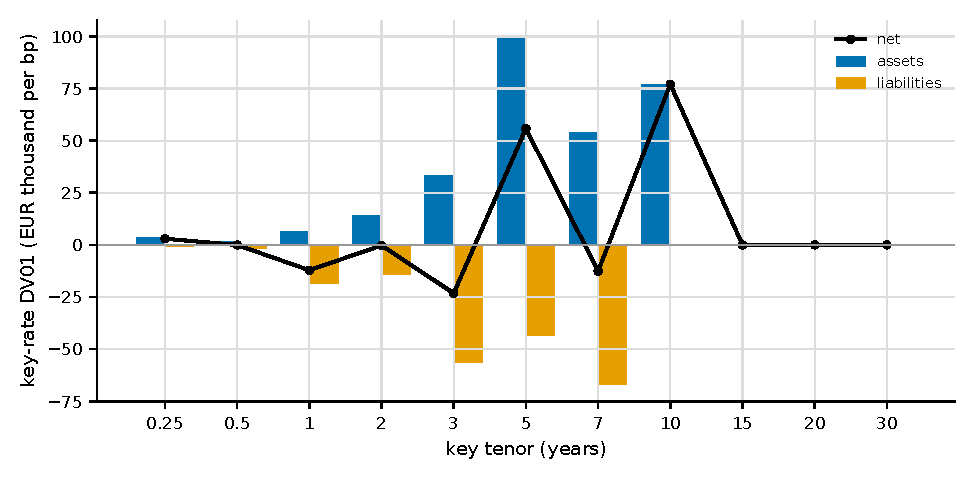
\includegraphics[width=\linewidth]{figures/fig15_key_rates.pdf}
\caption{Key-rate DV01 profile of the reference bank: value change for a 1 bp fall of the zero curve around each key tenor (tent-shaped bumps; the key rates sum to the parallel DV01). Assets gain, liabilities (negative cash flows) lose when rates fall; the net line is the bank's exposure.}
\label{fig:fig15_key_rates}
\end{figure}


\subsection{Model risk of the deposit assumptions}
\begin{figure}[H]
\centering
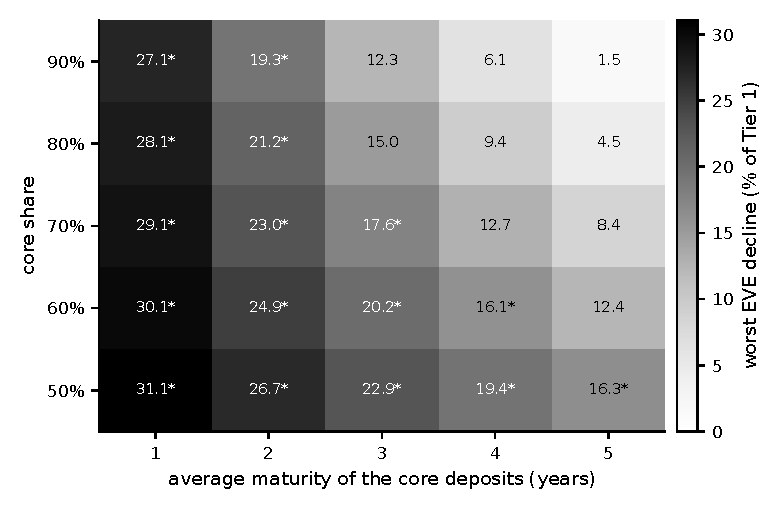
\includegraphics[width=0.75\linewidth]{figures/fig16_nmd_heat.pdf}
\caption{Model risk of the non-maturity-deposit assumptions: the worst EVE decline over the six scenarios (\% of Tier 1, BCBS 2016 EUR shocks) of the reference bank when the core share and the average maturity of the current-account deposits change (inside the caps). Only the current accounts (EUR 450\,m of the 600\,m non-maturity deposits) vary; the savings deposits keep their base assumptions. * = above the 15\,\% outlier threshold.}
\label{fig:fig16_nmd_heat}
\end{figure}

Within the caps for the core share and the average maturity, the same balance sheet passes or fails the EVE
outlier test depending only on the NMD assumptions.
\usertext{Which NMD assumption is supportable, and how would you validate it (deposit history, stress periods)?}

\subsection{Duration versus full revaluation}
\begin{figure}[H]
\centering
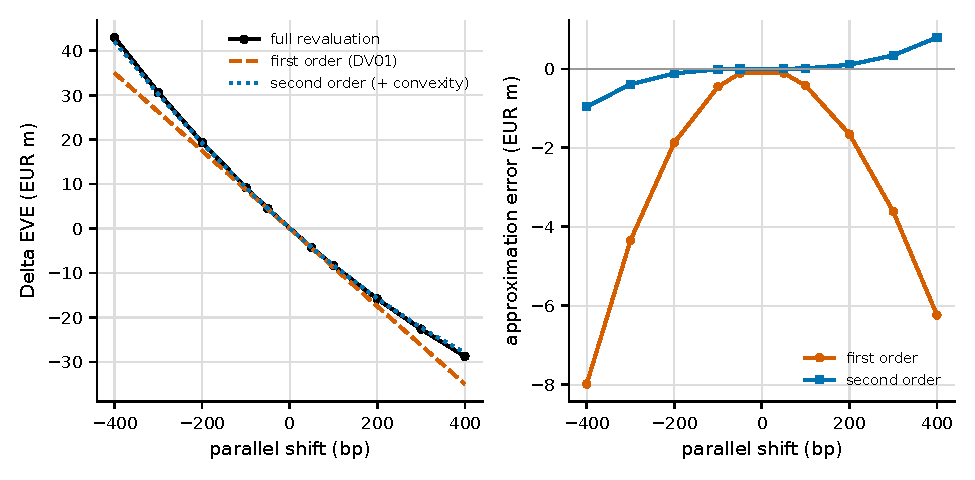
\includegraphics[width=\linewidth]{figures/fig17_duration_check.pdf}
\caption{Duration check on the reference bank: Delta EVE under parallel shifts (no floor) by full revaluation against the first-order (DV01) and second-order (DV01 + convexity) approximations. The first-order error grows with the square of the shift; the convexity term removes most of it.}
\label{fig:fig17_duration_check}
\end{figure}


% =====================================================================================
\section{Limitations}
\begin{itemize}
\item Synthetic bank and curve: the numbers illustrate the method, they do not describe a real bank.
\item Single currency, no credit spreads, no optionality beyond the deposit pass-through (no prepayments, no early
  redemption), instantaneous shocks, constant balance sheet for NII.
\item The NMD caps, marked ``ASSUMPTION'' in Table~\ref{tab:R3_assumptions}, must be checked against the primary
  texts before any use beyond this showcase.
\end{itemize}
\usertext{Further limitations the author sees.}

% =====================================================================================
\section{Findings}
\begin{table}[H]
\centering
\scriptsize
\caption{Findings register of the IRRBB study. Severities are PROPOSED and must be confirmed by the validator.}
\label{tab:R4_findings}
\setlength{\tabcolsep}{3pt}
\begin{tabular}{>{\raggedright\arraybackslash}p{0.75cm}>{\raggedright\arraybackslash}p{6.6cm}>{\raggedright\arraybackslash}p{1.85cm}>{\raggedright\arraybackslash}p{2.4cm}>{\raggedright\arraybackslash}p{3.5cm}}
\toprule
ID & Finding & Severity & Evidence & Proposed remediation \\
\midrule
R-F1 & The reference bank breaches the EVE outlier test: its worst EVE decline is 17.6\,\% of Tier 1 under parallel up (threshold 15\,\%); 19.6\,\% with the 2024 EUR shock sizes. The exposure comes from long fixed-rate assets (10-year mortgages and bonds) funded by short liabilities. & PROPOSED: High & Tab.~\ref{tab:R1_scenarios}, \ref{tab:R2_outlier_test}; Fig.~\ref{fig:fig14_irrbb_delta} & Hedge the long fixed-rate assets (payer swaps at the 5--10-year key rates, Fig.~\ref{fig:fig15_key_rates}). \\
R-F2 & The result depends on the non-maturity-deposit assumptions: with the core share and average maturity of the current accounts inside the caps, the worst EVE decline ranges from 1.5\,\% (90\,\% core, 5 years) to 31.1\,\% (50\,\% core, 1 year) of Tier 1; the base case (70\,\%, 3 years) gives 17.6\,\%. Only the current accounts (EUR 450\,m of the 600\,m non-maturity deposits) vary. The outlier test can be passed or failed by the NMD model alone. & PROPOSED: High & Fig.~\ref{fig:fig16_nmd_heat} & Treat the NMD model as a model with its own validation (deposit history, behavioural back-testing) and report the sensitivity with every EVE figure. \\
R-F3 & The bank also breaches the NII outlier test (6.4\,\% of Tier 1 under parallel down, threshold 5\,\%): deposit rates are floored at 0\,\% and cannot follow a fall in market rates, while floating-rate loans and reserves reprice down in full. The result depends on the 0\,\% deposit floor and the pass-through betas (0.3 current accounts, 0.5 savings). The short-down scenario, which the NII test does not use, is worse (-7.4\,\%). & PROPOSED: Medium & Tab.~\ref{tab:R1_scenarios}, \ref{tab:R2_outlier_test} & Review the deposit-floor and pass-through assumptions (beta); monitor NII under short-rate scenarios as well. \\
R-F4 & The breaches are robust to $\pm$30\,\% changes in the reference bank's composition (same NMD rates and betas, 0\,\% deposit floor, Tier 1 = 9\,\% of assets): of 2000 variants, 65.6 $\pm$ 1.1\,\% breach the EVE test and 96.7 $\pm$ 0.4\,\% the NII test (BCBS 2016 shocks). The NII breach is structural: floored deposits against fully repricing floating-rate loans and reserves. & PROPOSED: Medium & Tab.~\ref{tab:R2_outlier_test} & Treat the variants as a robustness check of the synthetic design, not as a population of real banks; for a real bank, analyse the deposit floor and pass-through instead. \\
R-F5 & A duration (DV01) approximation misstates Delta EVE for large shocks: at +200 bp it gives -17.5 against -15.8 EUR m by full revaluation; adding convexity gives -15.7. & PROPOSED: Low & Fig.~\ref{fig:fig17_duration_check} & Compute regulatory scenarios by full revaluation; use DV01 / key rates for limits and hedging only. \\
R-F6 & One parameter set could not be verified against a primary text: the BCBS caps on the core share and the average maturity of non-maturity deposits (marked ASSUMPTION in the register). The shock shapes and sizes, the floor and its rule for rates below it, and both outlier thresholds are cited to their articles. & PROPOSED: Low & Tab.~\ref{tab:R3_assumptions} & Verify the NMD caps against BCBS SRP31 (and the EU rules) before any use beyond this showcase. \\
\bottomrule
\end{tabular}
\end{table}


\section{Assumptions register}
\begin{table}[H]
\centering
\scriptsize
\caption{Assumptions register: every modelling choice and parameter source the results carry (``ASSUMPTION'' = not verified against a primary source in this work; ``verify'' = taken from a secondary source).}
\label{tab:R3_assumptions}
\setlength{\tabcolsep}{3pt}
\begin{tabular}{>{\raggedright\arraybackslash}p{3.0cm}>{\raggedright\arraybackslash}p{10.6cm}>{\raggedright\arraybackslash}p{2.1cm}}
\toprule
Item & Statement and source & Status \\
\midrule
EVE & run-off cash flows, equity excluded, single currency (no 50 \% weight on gains across currencies) & sourced \\
FRN & reprices to par at the next reset; margins after it are excluded from EVE & sourced \\
NII horizon & 12 months, monthly grid, constant balance sheet, instantaneous shock & sourced \\
NMD caps & BCBS (2016) d368 table 2 / Basel Framework SRP31, as recalled - ASSUMPTION (not verified against the primary text) & ASSUMPTION \\
NMD rate & pass-through beta on the 0.25-year zero-rate shock, floored at the rate floor & sourced \\
NMD replicating portfolio & non-core overnight; core in equal monthly tranches over 2 x average maturity & sourced \\
constant balance sheet & for NII, maturing / amortised / reset balances are replaced by the same product at the contractual rate plus the shock to the zero rate at its repricing tenor & sourced \\
discounting & every cash flow on the risk-free zero curve (no credit spreads); continuous compounding & sourced \\
floor below observed & observed rate below the floor -> the lower observed rate applies: EBA/RTS/2022/10 Art. 4(k) / 1(2) & sourced \\
post-shock floor & min(0, -150 bp + 3 bp x t) - -150 bp at immediate maturity, +3 bp a year, 0 from 50 years: EBA/RTS/2022/10 Art. 4(k) (Delegated Regulation (EU) 2024/856); applied to both shock presets (a choice of this study) & sourced \\
run-off & EVE on contractual run-off cash flows (principal + interest); equity excluded & sourced \\
shock flattener & +0.8 |short| - 0.6 |long|: EBA/RTS/2022/10 Art. 3(d) (Delegated Regulation (EU) 2024/856) & sourced \\
shock shapes & short e\textasciicircum{}\{-t/4\}, long 1 - e\textasciicircum{}\{-t/4\}: BCBS d368 annex 2 / SRP31.91; checked against d578 & sourced \\
shock sizes EUR\_BCBS2016 & EUR\_BCBS2016: \{'parallel': 200.0, 'short': 250.0, 'long': 100.0\} bp - BCBS (2016) d368, annex 2, table of specified shocks: EUR 200 / 250 / 100 bp & sourced \\
shock sizes EUR\_BCBS2024 & EUR\_BCBS2024: \{'parallel': 225.0, 'short': 350.0, 'long': 200.0\} bp - BCBS (2024) d578 recalibration (16 July 2024, effective 1 January 2026): EUR 225 / 350 / 200 bp & sourced \\
shock steepener & -0.65 |short| + 0.9 |long|: checked against the worked example in d578 (SRP31.92) & sourced \\
\bottomrule
\end{tabular}
\end{table}


\section*{References}
\begin{itemize}
\item Basel Committee on Banking Supervision (2016). \emph{Interest rate risk in the banking book} (standards, d368).
\item Basel Committee on Banking Supervision (2024). \emph{Recalibration of shocks for interest rate risk in the
  banking book} (d578).
\item European Banking Authority (2022). Regulatory technical standards on supervisory outlier tests
  (EBA/RTS/2022/10), adopted as Commission Delegated Regulation (EU) 2024/856; EBA Opinion of 26 April 2023 on the
  NII outlier test.
\item Directive 2013/36/EU (CRD), Art.~98(5).
\item Nelson, C. R. and Siegel, A. F. (1987). Parsimonious modeling of yield curves. \emph{Journal of Business}
  60(4), 473--489.
\item Svensson, L. E. O. (1994). Estimating and interpreting forward interest rates: Sweden 1992--1994. NBER
  Working Paper 4871.
\item Diebold, F. X. and Li, C. (2006). Forecasting the term structure of government bond yields. \emph{Journal of
  Econometrics} 130(2), 337--364.
\end{itemize}

\appendix
\section{Reproduction}
From \texttt{UFOS.ai/RiskLab/}:
\begin{verbatim}
python studies/irrbb_scenarios.py --mode full --save-results
python report/build_report.py --doc irrbb
# -> out/report/irrbb.pdf
\end{verbatim}

\end{document}
